\section{Analysis}
	\subsection{Theoretical}
	
	\subsection{Empirical}

		\begin{frame}{Baselines}
		\textbf{Algorithms used for comparisons}
		\begin{itemize}
			\item[$\bullet$] \textbf{balanced quantum k-means} (case study)
			\item[$\bullet$] \textbf{balanced classical k-means} (authors implementation)
			\item[$\bullet$] \textbf{classical k-means} (scikit-learn implementation)
		\end{itemize}

		classical k-means is a \textbf{valid comparison}

		% the above algorithms are the three baselines used
		% classical version of the k-means (non balanced) is used since, due to the structure 
		% of the dataset, constitute a valid comparison.
		
		\end{frame}

		\begin{frame}{Performance Metrics}
						
			\textbf{Adjusted Rand Index (ARI)}
			\begin{itemize}
				\item[$\bullet$] compare the similarity of two partitions of a dataset
				\item[$\bullet$] range from $-1$ to $1$ 
				\item[$\bullet$] used to compare \textbf{target partitions} vs \textbf{clustering partitions} 
			\end{itemize}
			
			\textbf{Total Computing time in quantum approach}
			\begin{equation}
				t = t_{QUBO_convertion} + t_{e} + t_{a} + t_{postprocessing}
			\end{equation}

			% here we have 2 metrics for the comparison, the ARI is and indicator
			% of similarity between 2 partitions, it ranges between -1 and 1 
			% high values indicates high similarity, 0 means random assignment
			% and in the paper is used to compare the target partition (correct solution)
			% with the one obtained by the cluster
			% the second metric is the tot computing time, this metric in quantum approach
			% is fragmented in different time measures:
			% $t_{QUBO convertion}$ time to convert the problem in QUBO
			% $t_{e}$ time to embed the QUBO on hardware 	
			% $t_{a}$ time to solve the QUBO (anealing time)
			% $t_{postprocessing}$ extract clustering from binary solution
		
		\end{frame}

		\begin{frame}{Data Generation}

			synthetic classification datasets created with \textit{make\_classification} (Scikit-learn)	\\
			\textbf{Datasets structure}
			\begin{itemize}
				\item[$\bullet$] \textbf{N} points	
				\item[$\bullet$] \textbf{k} classes	
				\item[$\bullet$] \textbf{1} cluster per class	
				\item[$\bullet$] \textbf{d} features 
				\item[$\bullet$] clusters \textbf{centered} on a \textit{d}-dimensional hypercube (with side length $2.0$)  
				\item[$\bullet$] points generated from a \textbf{normal dist.} about their cluster center (std $1.0$)   
				\item[$\bullet$] each class made of $\frac{N}{k}$ \textbf{points}   
			\end{itemize}

			% data for experiments is generated from a scikit learn function called make_classification
			% for each experiments, as we will see later 50 datasets are created with the following characteristics
			% * description of the list *
			
		\end{frame}

		\begin{frame}{Experiments' Hardware Configuration}	
			\textbf{Classical Machine}
			\begin{itemize}
				\item[$\bullet$] 2.7 GHz Dual-Core Intel i5 
				\item[$\bullet$] 8 GB 1.867 MHz DDR3 memory 
			\end{itemize}

			\textbf{Quantum Machine}
			\begin{itemize}
				\item[$\bullet$] D-Wave 2000Q quantum computer 
				\item[$\bullet$] 2048 qubits, 5600 inter-qubit connections
			\end{itemize}

			\textbf{Technical Aspects}
			\begin{itemize}
				\item[$\bullet$] \textbf{quantum pre/post-processing} done via the above \textbf{classical} machine
				\item[$\bullet$] quantum \textbf{anealing} operation \textbf{perfomed 100 times} for each experiment   
				\item[$\bullet$] only ground state is used % TODO: find out the meaning  
			\end{itemize}			

			% the Hardware used for the experiments is reported in this slide
			% * description of the list *
			% what it means with only ground state is used???

		\end{frame}

		\begin{frame}{Experiments}
			\textbf{Experiments Setup}
			\begin{itemize}
				\item[$\bullet$] clustering quality of the 3 algorithms is compared
				\item[$\bullet$] each algorithm evaluated on different \textbf{problem types}
				\begin{itemize}
					\item[$\circ$] total of 9 problem types 
					\item[$\circ$] defined by \textit{(num. of points, num. of clusters)}
				\end{itemize}
				\item[$\bullet$] for each problem type:
				\begin{itemize}
					\item[$\circ$]  all the 3 algorithm evaluated on 50 \textbf{synthetic datasets}
				\end{itemize}
			\end{itemize}

			% the experiments are carried for different problem types, problem type are
			% defined by the number of points and number of clusters for instance (12, 3)
			% the main experiment is done with 9 problem types, for each of them 
			% the algorithms are evaluated on the 50 generated datasets
			
		\end{frame}

		\begin{frame}{Experiments}
			\textbf{Commenting Results for Quantum Approach}
			\begin{itemize}
				\item[$\bullet$] performances drop for $k=2$
				\begin{itemize}
					\item[$\circ$] less way to cluster $\Longrightarrow$ local solution is more likely to be the correct one 
				\end{itemize}
				\item[$\bullet$] performances drop as the problem size increase 
				\begin{itemize}
					\item[$\circ$] reflection of the quantum hardware
				\end{itemize}
				%\item[$\bullet$] best performances obtained for problem types (8,4) (12, 3) (12, 4)  
			\end{itemize}

			\begin{center}
				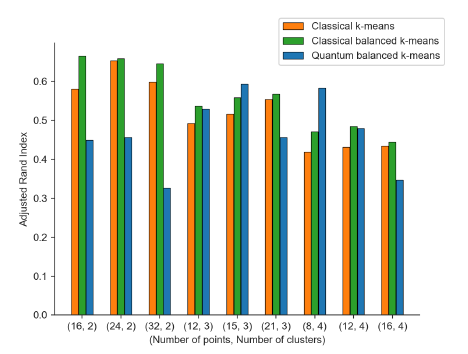
\includegraphics[scale=0.65]{first_ARI_table.png}
			\end{center}

			% * same things in the slides *
		\end{frame}

		\begin{frame}[allowframebreaks]{Limitations and Approximations}
			\textbf{Limitations faced}
			\begin{itemize}
				\item[$\bullet$] \textbf{Variable limitation} D-Wave 2000Q qubit limitation for problems $Nk > 64$ var.
				\item[$\bullet$] \textbf{Qubit connectivity} "limitation" $=>$ higher embedding time
			\end{itemize}
			\textbf{Approximations}
			\begin{itemize}
				\item[$\bullet$] Quantum run time for larger problems ($Nk > 64$)
				\begin{itemize}
					\item[$\circ$] used to evaluate scalability of the Quantum Approach
					\item[$\circ$] measure $t_{QUBO_convertion}$ (measurable)
					\item[$\circ$] estimate embedding time $t_{e}$ (from smaller problems)
					\item[$\circ$] estimate annealing time $t_{a}$ (constant, averaging smaller problems) 
					\item[$\circ$] measure $t_{postprocessing}$
				\end{itemize} 
			\end{itemize}
			embedding algorithms chosen \textbf{scales quadratically} in the number of \textbf{binary variables} of the QUBO
			\begin{equation}
				t_{e} = 1.887 \times 10^{-6}(Nk)^2 
				+ 4.632 \times 10^{-6}(Nk)
				+ 4.022 \times 10^{-4}
			\end{equation}
			\begin{equation}
				t_{a} = 0.03481 \pm 0.00008
			\end{equation}

			% here the main limitations are about variables, since D-Wave 2000Q can't handle problems with more than 64 variables
			% and the qubit connectivity, of course the more the connections the more time is required by the embedding algorithm
			% approximation introduced is the evaluations for problems with more than 64 variables, since we cannot test them in
			% practice, to estimate the new computing time we have to approximate the anealing time and the embedding time, other 
			% values are measurable, since they happen in classical. since the embedding algorithm choosed by authors scale quadratically
			% in num of var can be approx with this formula. for what concern the anealing time, since it is costant one measured
			% in previous examples is used
		\end{frame}

		\begin{frame}{Scalability}
			\textbf{Experiments to assess scalability}
			\begin{itemize}
				\item[$\bullet$] baselines evaluated on the three variables:
				\begin{itemize}
					\item[$\circ$] $N$ data points  					
					\item[$\circ$] $k$ clusters
					\item[$\circ$] $d$ features 
				\end{itemize}
				\item[$\bullet$] $\forall$ \textbf{problem type} baselines runned on 50 \textbf{synthetic datasets}
			\end{itemize}

			% * same things in the slides *
		\end{frame}

		\begin{frame}[allowframebreaks]{Scalability w.r.t. points (N)}
			\textbf{Setup and Considerations}
			\begin{itemize}
				\item[$\bullet$] baselines evaluated on increasing \textbf{data points}
				\item[$\bullet$] fixed cluster $k=4$ and features $d=2$
				\item[$\bullet$] considerations:
				\begin{itemize}
					\item[$\circ$] quantum is outperformed (due to embedding time)
					\item[$\circ$] future embedding time improvements may surpass classical balanced ($N \geq 1024$)
					\item[$\circ$] classical k-means scales the best expected since its \textbf{time complexity} $O(Nkd)$ vs quantum balanced $O(N^2kd)$ 
				\end{itemize} 
			\end{itemize}
			\begin{center}
				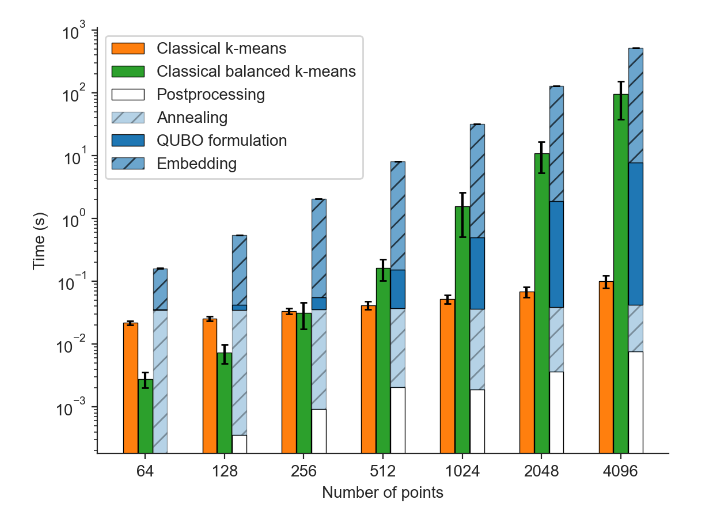
\includegraphics[scale=0.35]{scalability_points.png}
			\end{center}	
			
			% * same things in the slides *
		\end{frame}

		\begin{frame}[allowframebreaks]{Scalability w.r.t. clusters (k)}
			\textbf{Setup and Considerations}
			\begin{itemize}
				\item[$\bullet$] baselines evaluated on increasing \textbf{cluster size}
				\item[$\bullet$] fixed data points $N=256$ and features $d=8$
				\item[$\bullet$] considerations:
				\begin{itemize}
					\item[$\circ$] quantum scales worse on cluster size w.r.t. to other approaches
					\item[$\circ$] expected: third term on QUBO has $O(Nk^2)$ time complexity
				\end{itemize} 
			\end{itemize}
			\begin{center}
				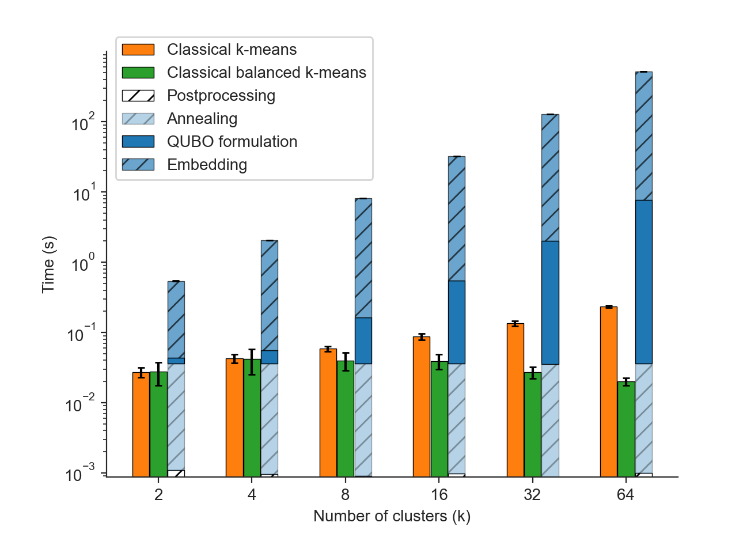
\includegraphics[scale=0.35]{scalability_clusters.png}
			\end{center}
			% * same things in the slides *
		\end{frame}

		\begin{frame}[allowframebreaks]{Scalability w.r.t. features (d)}
			\textbf{Setup and Considerations}
			\begin{itemize}
				\item[$\bullet$] baselines evaluated on increasing \textbf{features number}
				\item[$\bullet$] fixed data points $N=1024$ and cluster $k=4$ 
				\item[$\bullet$] considerations:
				\begin{itemize}
					\item[$\circ$] quantum is the worse on time 
					\item[$\circ$] quantum is promising in a future perspective, depending on embedding process optimizations
					\item[$\circ$] quantum approach scales better w.r.t. to classical \textit{k-means} on $d$  
					\item[$\circ$] expected: QUBO formulation only requires one comput. related to the dimension of the dataset % TODO: check this better 
					\item[$\circ$] \textit{classical balanced k-means} scales better in $d$ w.r.t. to quantum approach 
					\item[$\circ$] expected: \textit{quantum balanced} $O(N^2kd)$ vs \textit{classical balanced} $O(N^3)$  
				\end{itemize} 
			\end{itemize}
			\begin{center}
				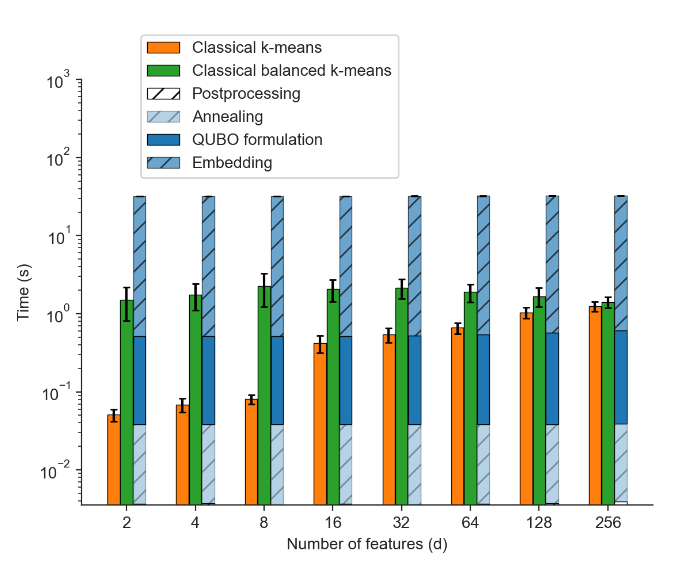
\includegraphics[scale=0.35]{scalability_features.png}
			\end{center}
			% * same things in the slides *
		\end{frame}
	
	\subsection{Benchmark}
	\begin{frame}[allowframebreaks]{Clustering a Benchmark Data Set}
		\textbf{The Iris Dataset}
		\begin{itemize}
			\item[$\bullet$] Reduced due to qubit limitations on modern hardware
			\item[$\bullet$] Pick $N/k$ points from $2\leq k \leq3$ of the data set's classes
		\end{itemize}
	
		\textbf{Experiments Run}
		\begin{itemize}
			\item[$\bullet$] All the 3 clustering algorithms were tested
			\item[$\bullet$] Experiments are run on 50 subsets of the dataset
		\end{itemize}
	
		\textbf{Results}
		\begin{itemize}
			\item[$\bullet$] $k=2$
			\begin{itemize}
				\item[$\circ$] Trivial case, points are linearly separable
				\item[$\circ$] Classical algorithms perform better than quantum
				\item[$\circ$] Evident as the number of binary variables $(Nk)$ increases
			\end{itemize}
			% Iris dataset used as proof of consistency of the previous results on a typical benchmarck dataset
			% Even if the dataset is composed of just 150 points with 4 features and k classes the quantum algorithm is still not powerful enough
			% Hence they reduced the number of points to N/k and considered k between 2 and 3
			% Results for k = 2 are significantly better for the classical algorithms since points are linearly separable and the global optimum is always found
		
			\framebreak
			\item[$\bullet$] $k=3$
			\begin{itemize}
				\item[$\circ$] Similar performance to \textbf{classical balanced} k-means
				\item[$\circ$] Outperforms \textbf{Scikit-Learn} implementation
				\item[$\circ$] Performance of the QA degrades as the problem size increases
			\end{itemize}
		\end{itemize}
		\begin{center}
			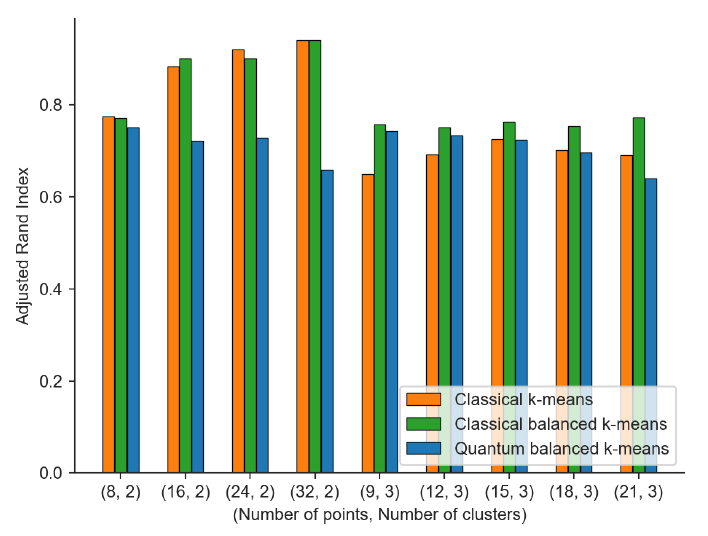
\includegraphics[scale=0.45]{Iris_ARI_table.png}
		\end{center}
		% For k = 3 the quantum algorithm performs as well as the classical balanced k-means and outperforms Scikit-learn implementation
		% The ARI table for this last experiments shows the results obtained and makes evidence that when the size of the problem increases, the performances of the QA degrade
	\end{frame}